\documentclass[]{article}
\usepackage[T1]{fontenc}
\usepackage{lmodern}
\usepackage{amssymb,amsmath}
\usepackage{ifxetex,ifluatex}
\usepackage{ctan}
\usepackage{tikz}
\usepackage{graphicx}
\usepackage{fixltx2e} % provides \textsubscript
% use upquote if available, for straight quotes in verbatim environments
\IfFileExists{upquote.sty}{\usepackage{upquote}}{}
\ifnum0\ifxetex1\fi\ifluatex1\fi=0 % if pdftex
  \usepackage[utf8]{inputenc}
\else % if luatex or xelatex
  \ifxetex\usepackage{mathspec}
    \usepackage{xltxtra,xunicode}
  \else
    \usepackage{fontspec}
  \fi
  \defaultfontfeatures{Mapping=tex-text,Scale=MatchLowercase}
  \newcommand{\euro}{€}
\fi
% use microtype if available
\IfFileExists{microtype.sty}{\usepackage{microtype}}{}
\ifxetex\usepackage[setpagesize=false, % page size defined by xetex
              unicode=false, % unicode breaks when used with xetex
              xetex]{hyperref}
\else
  \usepackage[unicode=true]{hyperref}
\fi
\hypersetup{breaklinks=true,
            bookmarks=true,
            pdfauthor={},
            pdftitle={},
            colorlinks=true,
            citecolor=blue,
            urlcolor=blue,
            linkcolor=magenta,
            pdfborder={0 0 0}}
\urlstyle{same}  % don't use monospace font for urls
\setlength{\parindent}{0pt}
\setlength{\parskip}{6pt plus 2pt minus 1pt}
\setlength{\emergencystretch}{3em}  % prevent overfull lines
\setcounter{secnumdepth}{0}

\author{}
\date{}

\begin{document}
\section{Examples}\label{examples}

\subsection{Synthesis of Collision Avoidance
Protocol}\label{synthesis-collision-avoidance-protocol}

\subsubsection{Problem statement}\label{problem-statement}

In this scenario we have $n$ UAVs, $m$ altitude layers and $q$ locations of
interest. A UAV can ascend or descend to the altitude layer above or
below its current altitude layer. A location is a predefined
point on an altitude layer. Our aim is to automatically synthesize a
control protocol that guarantees that each UAV is able to visit, infinitely
often, all of the locations of interest. Additionally, there must be no collision 
between UAVs.

\subsubsection{Approach}\label{approach}
Our approach to this problem is centered around the idea of UAVs'
operating regions. An operating region for a UAV is a polygon on the
UAV's current altitude layer. We assume That the UAV will only fly
within its operating region. With this assumption, we can guarantee that
no collision will happen if the UAV with intersected operating region
remain still until the intersection is resolved.

At each turn, each UAV will signal an intention to visit a specific location 
or to remain still. We assume that there cannot be two UAVs intending to fly 
to the same location to prevent deadlocks. We use this intention signal to update 
the operating regions for all the UAVs so that the intended locations are inside 
the operating regions of the UAVs. The algorithm for updating the operating regions 
ensures that the updated regions for all the UAVs do not intersect. Currently, there 
is no guarantee that the algorithm will terminate. The algorithm includes reshaping 
the operating regions and moving the UAVs to nearby location to resolve operating 
regions intersections. The UAV will then be given the command to fly to location it 
intended to fly to. It is assumed that the UAV will reach the location in one time step. 

\subsubsection{Problem setup}\label{problem-setup}
We model this problem by assigning three output variables, $l_{i} \in L$ for the layer 
that UAV$_{i}$ should ascend or descend to, where $L$ is the set of indices of the 
altitude layers, $t_{i} \in P$ for signaling UAV$_{i}$'s intended location to fly to, where $P$ 
is the set of indices of locations and $p_{i},t_{i} \in P$ for the location that UAV$_{i}$ should fly 
to. In addition, we assign $(n-1)^{2}$ input variables $c_{ij} \in B$, $i \neq j$ for indicating
whether the operating region of UAV$_{i}$ intersects with the operating region of
UAV$_{j}$, where $B$ is the boolean set and $n$ is the number of UAVs and $i,j \in U$, 
which is the set of indices for the UAVs.

\iffalse
\begin{itemize}
\item
  \textbf{$l_{i}$:} the altitude layer for UAV$_{i}$ to ascend or descend to.
\item
  \textbf{$p_{i}$:} the location for UAV$_{i}$ to head to.
\item
  \textbf{$t_{i}$:} the intention of  UAV$_{i}$.
\item
  \textbf{$c_{ij}$:} true if the operating region for
  UAV$_{i}$ intersects with that of UAV$_{j}$ and false otherwise.
\end{itemize}
\fi

\begin{figure}[htp]
\begin{tikzpicture}
    \node[anchor=south west,inner sep=0] (image) at (0,0,0) {\frame{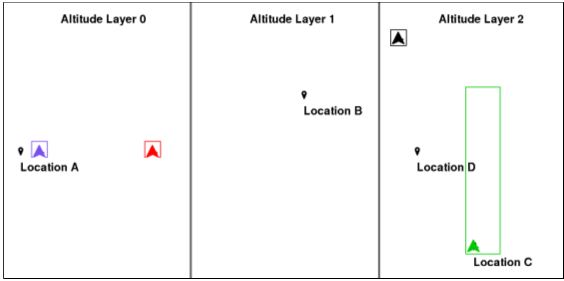
\includegraphics[width=5in]{figs/ca_1.png}}};
    \begin{scope}[x={(image.south east)},y={(image.north west)}]
    \end{scope}
\end{tikzpicture}
    \label{fig:ca}
    \caption{The airspace is divide into three equal layers numbered 0 to 2. Each
of the four UAVs has a polygon surrounding it with the same color which defines
the borders of the operating region of the UAV. The pinpoints point at the exact 
position of the corresponding location.}
\end{figure}


\subsubsection{System specifications}\label{system-specifications}

We express the system's specifications in four sets of LTL specifications. 
First, UAV$_{i}$ can only go to the locations that are in the same altitude layer $(\bigwedge\limits_{i \in U} \square (l_{i} = 
u \implies \bigvee\limits_{j\in C_{v}} p_{i} = v_{j} \lor p_{i} = \text{stay}))$ where $C_{v}$ is the set of indices of the
locations defined on the altitude layer $u$. Second, UAV$_{i}$ and UAV$_{j}$ must not 
be at the same altitude layer if $c_{ij}$ is true (their operating regions intersect!) 
$(\bigwedge\limits_{i\in U} \bigwedge\limits_{j\in U} \square (c_{ij} \implies l_{i} \neq l_{j}))$. Third, If UAV$_{i}$ is given a command to go 
to $x$ then it must have signaled its intent to do so at previous step 
$(\bigwedge\limits_{i \in U} \square (p_{i} = x \implies t_{i} = x))$. Lastly, UAV$_{i}$ will be repeatedly sent the command to fly over $x$ $(\bigwedge\limits_{i \in U} \square \lozenge (p_{i} = x))$.

\subsubsection{Environment assumptions}\label{environment-assumptions}


We assume that if two UAVs have intersecting operating regions ($c_{ij}$ is true) and 
one of the UAVs signaled an intention to go to a location then the intersection 
will be resolved ($c_{ij}$ is false).


\subsection{Synthesis of VIP Escort Protocol}\label{vip-escort}

\subsubsection{Problem statement}\label{problem-statement}

In this scenario we have one main UAV we call ``VIP'', multiple ``escort'' UAVs, 
and multiple pre-defined locations on the map. These locations are shown in 
green in fig \ref{fig:vip}. Our aim is to automatically synthesize a control protocol that 
guarantees the following three properties. First, The VIP must not fly from one 
location to another without being followed by one of the escorts. Second, The VIP 
cannot visit certain locations until at least one of the escorts have inspected the 
location within the last $x$ steps. A location is considered inspected if an escort 
flies over the location. In order for the UAVs not to pass through the prohibited 
regions shown in red in fig \ref{fig:vip}, the UAVs must follow certain paths between the 
locations in green. For example, to go from the bottom right location to the 
upper right, the UAVs must pass through the middle location so that they do not fly 
over the prohibited regions.

\begin{figure}[htp]
    \centering
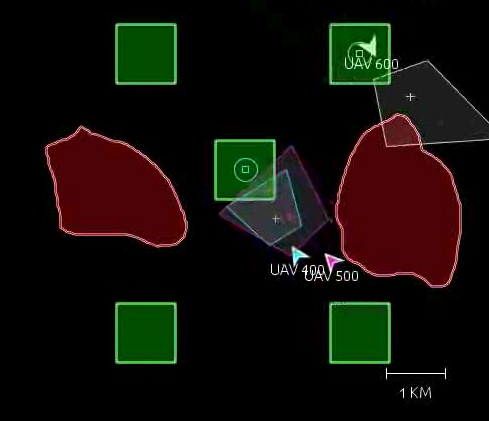
\includegraphics[scale=.4]{figs/vip.png}
    \caption{The escort UAV (purple) is tracking the VIP (blue), allowing the VIP
to fly from the bottom right location to the top right via the middle location.}
    \label{fig:vip}
\end{figure}


\subsubsection{Problem setup}\label{problem-setup}

We model this problem by assigning two output variables and one input variable
for the escort UAVs. $g_{i} \in P$ is an output variable that indicates the location that UAV$_{i}$ 
should fly to where $P$ is the set of location indices and $t_{i}\in B$, the second output 
variable, is an indicator for whether the escort UAV$_{i}$ should track the VIP or not, 
where $B$ is the boolean set and one input variable $s_{i} \in P$ for the current location 
of UAV$_{i}$ where $i \in U$, the set of escort UAV indices. As for the VIP, we assign 
one input variable $p \in P$ for the VIP's current location and one output variable 
$q \in P$ for the location that the VIP should fly to. In addition, we assign the
input variables $r_{i} \in B$ that indicate if the location was previously 
inspected.

\subsubsection{System specifications}\label{system-specifications}
The system specifications for synthesizing the controller consist of four 
sets of LTL specifications. First, the escort must be at the same location as the 
VIP to be able to begin tracking it $\square (t_{i} \implies p = s_{i})$. Secondly, The VIP 
cannot fly from a location to another without being followed by another UAV 
$\square(\bigwedge\limits_{i\in U}\lnot ti_{i} \implies \Circle p = p$). The third specification is that the VIP must always 
eventually visits a set of locations: $\bigwedge\limits_{p\in P}\square \lozenge q$. Lastly, a set of locations must 
always eventually be inspected $\bigwedge\limits_{i\in P}\square \lozenge r_{i}$.

\subsubsection{Environment assumptions}\label{environment-assumptions}
We express the environment's assumptions in three sets of LTL specifications. 
First, the location is considered inspected when an escort visits the location $\square (s_{i} \implies r_{i})$. Second, 
an inspected location remains inspected $\square (r_{i} \implies \Circle r_{i})$. It is also possible 
to set an expiration timer for the location to switch back not inspected. The 
last assumption is that all UAVs will reach their destinations that they were 
commanded to fly to by the next time step: $\square (g_{i} \implies \Circle s_{i})$.

\end{document}









